

\tikzset{every picture/.style={line width=0.75pt}} %set default line width to 0.75pt        

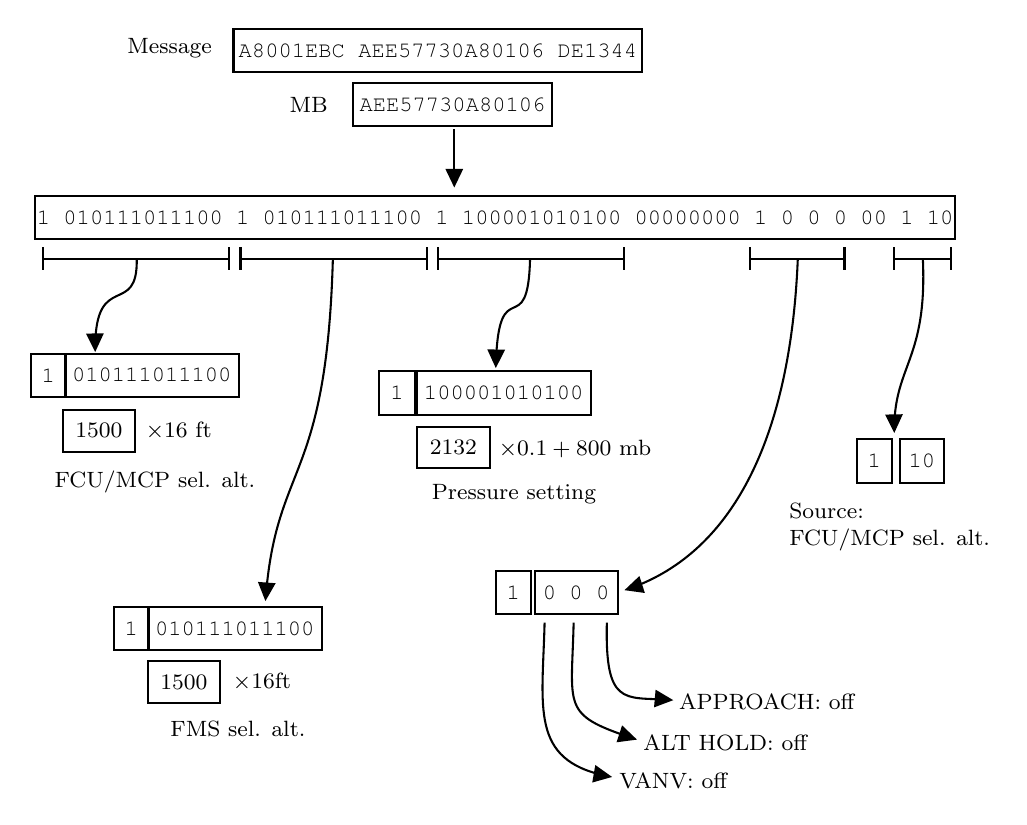
\begin{tikzpicture}[x=0.75pt,y=0.75pt,yscale=-1,xscale=1]
%uncomment if require: \path (0,432); %set diagram left start at 0, and has height of 432

%Curve Lines [id:da5981577463459831] 
\draw    (79,134.33) .. controls (79.57,162.77) and (59.38,139.8) .. (58.99,176.32) ;
\draw [shift={(59,179.25)}, rotate = 269.06] [fill={rgb, 255:red, 0; green, 0; blue, 0 }  ][line width=0.08]  [draw opacity=0] (8.93,-4.29) -- (0,0) -- (8.93,4.29) -- cycle    ;
%Curve Lines [id:da5084877796322058] 
\draw    (173.5,134.33) .. controls (170.45,242.9) and (146.49,231.49) .. (141.16,297.23) ;
\draw [shift={(141,299.25)}, rotate = 274.21] [fill={rgb, 255:red, 0; green, 0; blue, 0 }  ][line width=0.08]  [draw opacity=0] (8.93,-4.29) -- (0,0) -- (8.93,4.29) -- cycle    ;
%Curve Lines [id:da5650542056811212] 
\draw    (268.5,134.33) .. controls (267.52,175.49) and (253.57,139.5) .. (252.08,184.16) ;
\draw [shift={(252,187)}, rotate = 271.17] [fill={rgb, 255:red, 0; green, 0; blue, 0 }  ][line width=0.08]  [draw opacity=0] (8.93,-4.29) -- (0,0) -- (8.93,4.29) -- cycle    ;
%Curve Lines [id:da2826034018830037] 
\draw    (275.5,309.67) .. controls (274.52,350.62) and (268.32,375.72) .. (305.09,383.44) ;
\draw [shift={(308,384)}, rotate = 189.93] [fill={rgb, 255:red, 0; green, 0; blue, 0 }  ][line width=0.08]  [draw opacity=0] (8.93,-4.29) -- (0,0) -- (8.93,4.29) -- cycle    ;
%Curve Lines [id:da167001333387915] 
\draw    (289.5,309.67) .. controls (288.52,350.62) and (283.59,353.86) .. (317.33,365.12) ;
\draw [shift={(320,366)}, rotate = 198.12] [fill={rgb, 255:red, 0; green, 0; blue, 0 }  ][line width=0.08]  [draw opacity=0] (8.93,-4.29) -- (0,0) -- (8.93,4.29) -- cycle    ;
%Curve Lines [id:da03103602868349009] 
\draw    (305.5,309.67) .. controls (304.55,349.78) and (313.93,345.5) .. (334.51,346.78) ;
\draw [shift={(337.5,347)}, rotate = 185.04] [fill={rgb, 255:red, 0; green, 0; blue, 0 }  ][line width=0.08]  [draw opacity=0] (8.93,-4.29) -- (0,0) -- (8.93,4.29) -- cycle    ;
%Curve Lines [id:da5417401260605015] 
\draw    (457.75,134.33) .. controls (459.93,182.51) and (444.32,185.45) .. (443.99,215.39) ;
\draw [shift={(444,218.25)}, rotate = 268.83] [fill={rgb, 255:red, 0; green, 0; blue, 0 }  ][line width=0.08]  [draw opacity=0] (8.93,-4.29) -- (0,0) -- (8.93,4.29) -- cycle    ;
%Straight Lines [id:da924076364834967] 
\draw [line width=0.75]    (224,134.33) -- (313.6,134.33) ;
\draw [shift={(313.6,134.33)}, rotate = 180] [color={rgb, 255:red, 0; green, 0; blue, 0 }  ][line width=0.75]    (0,5.59) -- (0,-5.59)   ;
\draw [shift={(224,134.33)}, rotate = 180] [color={rgb, 255:red, 0; green, 0; blue, 0 }  ][line width=0.75]    (0,5.59) -- (0,-5.59)   ;
%Straight Lines [id:da1126730298431704] 
\draw [line width=0.75]    (129,134.33) -- (218.8,134.33) ;
\draw [shift={(218.8,134.33)}, rotate = 180] [color={rgb, 255:red, 0; green, 0; blue, 0 }  ][line width=0.75]    (0,5.59) -- (0,-5.59)   ;
\draw [shift={(129,134.33)}, rotate = 180] [color={rgb, 255:red, 0; green, 0; blue, 0 }  ][line width=0.75]    (0,5.59) -- (0,-5.59)   ;
%Straight Lines [id:da6889757950929192] 
\draw [line width=0.75]    (34,134.33) -- (123.6,134.33) ;
\draw [shift={(123.6,134.33)}, rotate = 180] [color={rgb, 255:red, 0; green, 0; blue, 0 }  ][line width=0.75]    (0,5.59) -- (0,-5.59)   ;
\draw [shift={(34,134.33)}, rotate = 180] [color={rgb, 255:red, 0; green, 0; blue, 0 }  ][line width=0.75]    (0,5.59) -- (0,-5.59)   ;
%Straight Lines [id:da5545710261355621] 
\draw [line width=0.75]    (374.5,134.33) -- (420,134.33) ;
\draw [shift={(420,134.33)}, rotate = 180] [color={rgb, 255:red, 0; green, 0; blue, 0 }  ][line width=0.75]    (0,5.59) -- (0,-5.59)   ;
\draw [shift={(374.5,134.33)}, rotate = 180] [color={rgb, 255:red, 0; green, 0; blue, 0 }  ][line width=0.75]    (0,5.59) -- (0,-5.59)   ;
%Straight Lines [id:da06655537350580443] 
\draw [line width=0.75]    (444,134.33) -- (471.5,134.33) ;
\draw [shift={(471.5,134.33)}, rotate = 180] [color={rgb, 255:red, 0; green, 0; blue, 0 }  ][line width=0.75]    (0,5.59) -- (0,-5.59)   ;
\draw [shift={(444,134.33)}, rotate = 180] [color={rgb, 255:red, 0; green, 0; blue, 0 }  ][line width=0.75]    (0,5.59) -- (0,-5.59)   ;
%Curve Lines [id:da6196785513080374] 
\draw    (397.5,134.33) .. controls (394.13,217.73) and (367.81,275.25) .. (316.37,293.21) ;
\draw [shift={(314,294)}, rotate = 342.22] [fill={rgb, 255:red, 0; green, 0; blue, 0 }  ][line width=0.08]  [draw opacity=0] (8.93,-4.29) -- (0,0) -- (8.93,4.29) -- cycle    ;
%Straight Lines [id:da65120732921535] 
\draw    (232,72) -- (232,97) ;
\draw [shift={(232,100)}, rotate = 270] [fill={rgb, 255:red, 0; green, 0; blue, 0 }  ][line width=0.08]  [draw opacity=0] (8.93,-4.29) -- (0,0) -- (8.93,4.29) -- cycle    ;

% Text Node
\draw    (125.63,23.5) -- (322.63,23.5) -- (322.63,44.5) -- (125.63,44.5) -- cycle  ;
\draw (224.13,34) node  [font=\footnotesize] [align=left] {{\fontfamily{pcr}\selectfont A8001EBC AEE57730A80106 DE1344}};
% Text Node
\draw (161.88,60) node  [font=\footnotesize] [align=left] {MB};
% Text Node
\draw    (30.2,104) -- (473.2,104) -- (473.2,125) -- (30.2,125) -- cycle  ;
\draw (251.7,114.5) node  [font=\footnotesize] [align=left] {{\fontfamily{pcr}\selectfont 1 010111011100 1 010111011100 1 100001010100 00000000 1 0 0 0 00 1 10}};
% Text Node
\draw    (183.13,49.5) -- (279.13,49.5) -- (279.13,70.5) -- (183.13,70.5) -- cycle  ;
\draw (231.13,60) node  [font=\footnotesize] [align=left] {{\fontfamily{pcr}\selectfont AEE57730A80106}};
% Text Node
\draw    (27.88,180) -- (44.88,180) -- (44.88,201) -- (27.88,201) -- cycle  ;
\draw (36.38,190.5) node  [font=\footnotesize] [align=left] {{\fontfamily{pcr}\selectfont 1}};
% Text Node
\draw    (44.26,180) -- (128.26,180) -- (128.26,201) -- (44.26,201) -- cycle  ;
\draw (86.26,190.5) node  [font=\footnotesize] [align=left] {{\fontfamily{pcr}\selectfont 010111011100}};
% Text Node
\draw    (43.26,207.25) -- (78.26,207.25) -- (78.26,227.25) -- (43.26,227.25) -- cycle  ;
\draw (60.76,217.25) node  [font=\footnotesize] [align=left] {1500};
% Text Node
\draw (81.87,217.25) node [anchor=west] [inner sep=0.75pt]  [font=\footnotesize] [align=left] {$\displaystyle \times 16$ ft};
% Text Node
\draw    (67.88,302) -- (84.88,302) -- (84.88,323) -- (67.88,323) -- cycle  ;
\draw (76.38,312.5) node  [font=\footnotesize] [align=left] {{\fontfamily{pcr}\selectfont 1}};
% Text Node
\draw    (84.26,302) -- (168.26,302) -- (168.26,323) -- (84.26,323) -- cycle  ;
\draw (126.26,312.5) node  [font=\footnotesize] [align=left] {{\fontfamily{pcr}\selectfont 010111011100}};
% Text Node
\draw    (84.26,328.25) -- (119.26,328.25) -- (119.26,348.25) -- (84.26,348.25) -- cycle  ;
\draw (101.76,338.25) node  [font=\footnotesize] [align=left] {1500};
% Text Node
\draw (123.87,338.25) node [anchor=west] [inner sep=0.75pt]  [font=\footnotesize] [align=left] {$\displaystyle \times 16${\fontfamily{pcr}\selectfont  }ft};
% Text Node
\draw    (195.88,188.5) -- (212.88,188.5) -- (212.88,209.5) -- (195.88,209.5) -- cycle  ;
\draw (204.38,199) node  [font=\footnotesize] [align=left] {{\fontfamily{pcr}\selectfont 1}};
% Text Node
\draw    (213.8,188.5) -- (297.8,188.5) -- (297.8,209.5) -- (213.8,209.5) -- cycle  ;
\draw (255.8,199) node  [font=\footnotesize] [align=left] {{\fontfamily{pcr}\selectfont 100001010100}};
% Text Node
\draw    (214.1,215.25) -- (249.1,215.25) -- (249.1,235.25) -- (214.1,235.25) -- cycle  ;
\draw (231.6,225.25) node  [font=\footnotesize] [align=left] {2132};
% Text Node
\draw (252,225.75) node [anchor=west] [inner sep=0.75pt]  [font=\footnotesize] [align=left] {$\displaystyle \times 0.1+800$ mb};
% Text Node
\draw (94.82,33) node  [font=\footnotesize] [align=left] {Message};
% Text Node
\draw    (425.88,221.33) -- (442.88,221.33) -- (442.88,242.33) -- (425.88,242.33) -- cycle  ;
\draw (434.38,231.83) node  [font=\footnotesize] [align=left] {{\fontfamily{pcr}\selectfont 1}};
% Text Node
\draw    (446.8,221.33) -- (467.8,221.33) -- (467.8,242.33) -- (446.8,242.33) -- cycle  ;
\draw (457.3,231.83) node  [font=\footnotesize] [align=left] {{\fontfamily{pcr}\selectfont 10}};
% Text Node
\draw    (251.88,284.67) -- (268.88,284.67) -- (268.88,305.67) -- (251.88,305.67) -- cycle  ;
\draw (260.38,295.17) node  [font=\footnotesize] [align=left] {{\fontfamily{pcr}\selectfont 1}};
% Text Node
\draw    (270.7,284.67) -- (310.7,284.67) -- (310.7,305.67) -- (270.7,305.67) -- cycle  ;
\draw (290.7,295.17) node  [font=\footnotesize] [align=left] {{\fontfamily{pcr}\selectfont 0 0 0}};
% Text Node
\draw (337.45,385.67) node  [font=\footnotesize] [align=left] {VANV: off};
% Text Node
\draw (362.53,367.33) node  [font=\footnotesize] [align=left] {ALT HOLD: off};
% Text Node
\draw (382.53,347.67) node  [font=\footnotesize] [align=left] {APPROACH: off};
% Text Node
\draw (441.76,263.67) node  [font=\footnotesize] [align=left] {Source:\\FCU/MCP sel. alt.};
% Text Node
\draw (87.76,241.67) node  [font=\footnotesize] [align=left] {FCU/MCP sel. alt.};
% Text Node
\draw (127.76,360.67) node  [font=\footnotesize] [align=left] {FMS sel. alt.};
% Text Node
\draw (260.76,247.67) node  [font=\footnotesize] [align=left] {Pressure setting};


\end{tikzpicture}
